\documentclass{article}

\usepackage{url}
\usepackage{color}
\usepackage{paralist}
\usepackage{fancyvrb}
\usepackage{amsmath}
\usepackage{epsfig}
\usepackage{subfig}
\usepackage{float}
\usepackage[nomove]{cite}
\usepackage{tabularx}
\usepackage[table]{xcolor}
\usepackage{amssymb}
\usepackage{mdframed}
\usepackage{graphicx}
\graphicspath{ {figures/} }   

\DeclareRobustCommand{\rchi}{{\mathpalette\irchi\relax}}
\newcommand{\irchi}[2]{\raisebox{\depth}{$#1\chi$}}

\newcommand{\new}[1]{{\color{blue}#1}}
\newcommand{\draft}[1]{{\color{red}#1}}
\long\def\comment#1{}
\newcommand{\q}[1]{\lq\lq{}{}#1\rq\rq{}{}}

\begin{document}

\title{
    A PageRank like Approach for Ranking Archived Documents for Structured Queries
}

\author{
    %Pavlos Fafalios\\
    %L3S Research Center\\
    %Leibniz Universit\"{a}t Hannover\\
    %Hannover, Germany\\
    %\texttt{fafalios@l3s.de}
    %\and
    Vaibhav Kasturia\\
    L3S Research Center\\
    Leibniz Universit\"{a}t Hannover\\
    Hannover, Germany\\
    \texttt{kasturia@l3s.de}
    }
    \date{\today}
\maketitle

    \tolerance=1
    \emergencystretch=\maxdimen
    \hyphenpenalty=10000
    \hbadness=10000

\section{Introduction}
\subsection{Notions and Notations}

{\bf Web Entities, Concepts and Events}.
In our problem, we define a {\em web entity} $e$ as anything with a 
distinct, separate and meaningful existence that also has a \q{web identity} which is expressed through a unique URI $u_e$(e.g., a Wikipedia/DBpedia URI).
This not only includes persons, locations, organizations, etc., but also
concepts (e.g., {\em liberty}) and events (e.g., {\em Iranian elections of 2012}).\footnote{From now on, when we say {\em entity} we refer to {\em entity}, {\em concept}, or {\em event}.}

Let $E$ be a finite set of web entities, e.g., all Wikipedia entities, concepts and events expressed through a set of URIs $U$.
Each entity $e \in E$ is associated with a unique URI, while several labels/names
can be used to refer to this entity.
For eg., for the entity {\em Donald Trump} (\url{https://en.wikipedia.org/wiki/Donald_Trump}),
possible names are \q{Donald Trump}, \q{Trump}, \q{President Trump}, etc.

\vspace{2mm} \noindent
{\bf Documents and extracted entities}.
Let $D$ be a set of documents, e.g., a set of news articles.
For a document $d \in D$, let $publ(d)$ denote its publication date.
Let also  $ents(d) \subseteq E$ be all entities mentioned in $d$.
%(actually the URIs of these entities\footnote{From now on, when we say \q{entity} we mean \q{web entity URI}.}).
Inversely, for an entity $e \in E$, let $docs(e) \subseteq D$
be all documents that mention $e$, i.e., $docs(e) = \{d \in D ~|~ e \in ents(d)\}$.
For an entity $e \in E$ and a document $d \in D$,
let $count(e, d)$ be the number of occurrences of $e$ in $d$.
%Now, let $ef(e, d) = \frac{count(e, d)}{\sum_{e' \in ents(d)}{count(e', d)}}$ be the
%(normalized) frequency of $e$ in $d$.
Finally, let $E_D$ be all entities mentioned in documents of $D$,
i.e., $E_D = \cup_{d \in D}{ents(d)}$.

\vspace{2mm} \noindent
{\bf Time periods}.
Let $\Delta$ be a fixed time period (e.g., {\em day}, {\em week} or {\em month}).
Based on a time period $\Delta$,
let $T = (t_0, t_1, \dots, t_n)$ be an ordered list of consecutive time points
covering the publication dates of all documents in $D$.
Note that $t_i - t_{i-1} = \Delta$, for each $i \geq 1$.
Now, let $\delta_i = [t_i, t_{i+1})$ be the time period of size $\Delta$ between two consecutive time points.
We consider that a document $d$ is published in the period $\delta_i$, if $t_i \leq publ(d) < t_{i+1}$.
For a document $d \in D$, let $timep(d)$ be the time period in which $d$ was published.
Now, let $P_D$ denote the set of distinct time periods of all documents in $D$,
i.e., $P_D = \cup_{d \in D}{\{timep(d)\}}$.
For a time period $p \in P_D$, let $docs(p) \subseteq D$ be the set of all
documents published within $p$, i.e., $docs(p) = \{d \in D ~|~ timep(d) = p\}$,
and $ents(p) \subseteq E_D$ be the set of
entities discussed in documents of $D$ published within $p$,
i.e., $ents(p) = \cup_{d \in docs(p)}{ents(d)}$.

\section{Problem Definition}
Given a corpus of documents $D$,
a set of entities $E_D$ mentioned in documents of $D$,
and a SPARQL query $Q$ requesting documents from $D$
published within a set of {\em time periods} $P_Q \subseteq P_D$ and
related to one or more {\em Entities of Interest (EoI)} $E_Q \subseteq E_D$
with logical {\tt AND} (mentioning all EoI) or {\tt OR} (mentioning at least one EoI) semantics,
and an RDF Graph $G$, 
the problem is how to rank the documents $D_Q \subseteq D$ that (equally) match the query $Q$ using a {\em PageRank-like algorithm}.

Figure \ref{fig:modelingExampleQ1} shows an example SPARQL query
requesting documents published in 1990
discussing about the entities {\em Nelson Piquet} %(\url{http://dbpedia.org/resource/Nelson_Piquet})
and {\em Ayrton Senna} %(\url{http://dbpedia.org/resource/Ayrton_Senna}).
({\tt AND} semantics),
while the query in Figure \ref{fig:modelingExampleQ2} requests
articles of 1990 discussing about {\em Ferrari Formula One drivers}
({\tt OR} semantics).


\begin{figure}[th]
\vspace{-4mm}
\centering \scriptsize
\begin{Verbatim}[frame=lines,numbers=left,numbersep=1pt]
SELECT DISTINCT ?article WHERE {
  ?article dc:date ?date FILTER(?date >= "1990-01-01"^^xsd:date &&
                                ?date <= "1990-12-31"^^xsd:date) .
  ?article oae:mentions ?entity1, ?entity2 .
  ?entity1 oae:hasMatchedURI  <http://dbpedia.org/resource/Nelson_Piquet> .
  ?entity2 oae:hasMatchedURI  <http://dbpedia.org/resource/Ayrton_Senna> }
\end{Verbatim}
\vspace{-5.5mm}
\caption{SPARQL query for retrieving articles of 1990 discussing
about {\em Nelson Piquet} and {\em Ayrton Senna} ({\tt AND} semantics).}
\label{fig:modelingExampleQ1}

%\vspace{-4mm}
\centering \scriptsize
\begin{Verbatim}[frame=lines,numbers=left,numbersep=1pt]
SELECT DISTINCT ?article WHERE {
  SERVICE <http://dbpedia.org/sparql> {
    ?p dc:subject <http://dbpedia.org/resource/Category:Ferrari_Formula_One_drivers> }
  ?article dc:date ?date FILTER(?date >= "1990-01-01"^^xsd:date &&
                                ?date <= "1990-12-31"^^xsd:date)
  ?article oae:mentions ?entity .
  ?entity oae:hasMatchedURI  ?p }
\end{Verbatim}
\vspace{-5.5mm}
\caption{SPARQL query for retrieving articles of 1990 discussing
about {\em Ferrari Formula One drivers} ({\tt OR} semantics).}
\label{fig:modelingExampleQ2}
\vspace{-4mm}
\end{figure}



\section{Probabilistic Analysis}
We {\em dynamically} construct a graph of documents and identified entities
and then analyze it probabilistically for identifying the important document
and entity nodes. 
For the graph analysis and its node scoring, we follow a 
Random Walk-based (PageRank-like) \cite
method because the theoretical framework is quite solid and also according to the 
need and application we can bias or customize the method.
The probabilistic analysis is mentioned in detail after we 
define some aspects and present an user side 
exploratory search scenario which better motivates the PageRank-like approach 
that we propose.

\subsection{Aspects}

We define the following aspects:
i) the {\em relativeness} of a document with respect to the EoI,
ii) the {\em timeliness} of a document with respect to its publication date, and
iii) the {\em relatedness} of a document with respect to its reference to other entities related to the EoI.
iii) the {\em time difference importance} between the publication dates of two documents.

\subsubsection*{Relativeness}

We consider that if the EoI are mentioned multiple times
within a document, the document should receive a high score
(since the document's topic may be about these entities).
The term frequency (in our case entity frequency) is a classic numerical statistic
that is intended to reflect how important
a word is to a document in a collection or corpus.

For the case of {\tt AND} semantics (\q{$\wedge$}),
the {\em relativeness} score of a document $d \in D_Q$ based only on the {\em frequency} of the EoI
is defined as:
\begin{equation}
\small
ScoreD^{f}_{\wedge}(d) = \frac{\sum_{e \in E_Q}{count(e, d)}}{\sum_{e' \in ents(d)}{count(e', d)}}
\end{equation}
Notice that the score of a document will be 1 if it contains the EoI and no other entity.

For the case of {\tt OR} semantics (\q{$\vee$}),
we can also consider the number of EoI mentioned in the document
(since a document does not probably contain all the EoI as in the case of {\tt AND} semantics).
In that case, the {\em relativeness} score can be defined as follows:
\begin{equation}
\small
ScoreD^{f}_{\vee}(d) = \frac{\sum_{e \in E_Q}{count(e, d)}}{\sum_{e' \in ents(d)}{count(e', d)}} \cdot \frac{|ents(d) \cap E_Q|}{|E_Q|}
\end{equation}
where $\frac{|ents(d) \cap E_Q|}{|E_Q|}$ is the percentage of EoI discussed in the document.
The score of a document will be 1 if it contains all the EoI and no other entity.
This formula favors documents mentioning multiple times many of the EoI.




\subsubsection*{Timeliness}

We consider that a time period $p \in P_Q$ is important
for the entities in $E_Q$, if there is a relatively big number of documents in $D_Q$
discussing about these entities during $p$.
For example, a big number of articles about {\em Nelson Mandela}
was published the period 11-13 of February 1990 because
in February 11 {\em Nelson Mandela} was released from prison.
Thus, articles published during that period should be promoted since
they are probably related to this important event of {\em Nelson Mandela}'s life.

For the case of {\tt AND} semantics,
we define the following importance score of a {\em time period} $p \in P_Q$:
\begin{equation}
ScoreP_\wedge(p) = \frac{|docs(p) \cap D_Q|}{|D_Q|}
\end{equation}
%Notice that this formula is actually a probability distribution
%for $p \ P_Q$ based on the EoI.

For the case of {\tt OR} semantics,
in a time period $p$ there may be a
big number of documents discussing only for one of the EoI,
while in a time period $p'$ there may be a smaller number
of documents discussing though for many of the EoI.
For also taking into account the number of EoI discussed in documents
of a specific time period, we consider the following formula:
\begin{equation}
\small
ScoreP_\vee(p) = \frac{|docs(p) \cap D_Q|}{|D_Q|} \cdot P_{EoI}(p)
% OLD: ScoreP_\vee(p) = \frac{|docs(p) \cap D_Q|}{|D_Q|} \cdot \frac{|ents(p) \cap E_Q|}{|E_Q|}
\end{equation}
where, $P_{EoI}(p)$ is the average percentage of EoI discussed in articles of $p \in P_Q$, i.e.:
\begin{equation}
\small
P_{EoI}(p) =  \frac{\sum_{d \in docs(p) \cap D_Q}{\frac{|ents(d) \cap E_Q|}{|E_Q|}}}{|docs(p) \cap D_Q|}
\end{equation}
By considering only timeliness,
the score of a document can be determined by the score
of its publication date, i.e.:

\begin{equation}
ScoreD^{t}(d) = ScoreP(timep(d))
\end{equation}

\subsubsection*{Relatedness}

Entities that are co-mentioned frequently with the EoI
in important time periods are probably important for the EoI.
For example, {\em Apartheid} was an important concept
related to {\em Nelson Mandela} %and {\em Frederik Willem de Klerk}
during 1990,
thus articles discussing for both {\em Apartheid} and {\em Nelson Mandela} %, and {\em Frederik Willem de Klerk}
should be promoted.
However, there may be also some general entities (e.g., {\em South Africa} in our example)
that co-occur with the EoI in almost all documents (independently of the time period).
Thus, we should also avoid over-emphasizing documents mentioning such \q{common} entities.
%(in a similar way to the computation of {\em tf-idf} in IR).

For the case of {\tt AND} semantics,
we consider the following {\em relatedness} score
for an entity $e \in E_D \setminus E_Q$:

\begin{equation}
\begin{split}
\small
ScoreE_\wedge(e) = & ~ idf_\wedge(e) \cdot \sum_{p \in P_Q}{(ScoreP_\wedge(p) \cdot \frac{|docs(p) \cap D_Q \cap docs(e)|}{|docs(p) \cap D_Q|})}\\
= & ~ idf_\wedge(e) \cdot \sum_{p \in P_Q}{\frac{|docs(p) \cap D_Q \cap docs(e)|}{|D_Q|}}
\end{split}
\end{equation}
where $idf_\wedge(e)$ is the inverse document frequency
of entity $e$ in the set of documents discussing about the EoI in the entire corpus,
which can be defined as follows:
\begin{equation}
\label{frml:idf_and}
\small
idf_\wedge(e) = 1 - \frac{|docs(e) \cap (\cap_{e' \in E_Q}{docs(e')})|}{|\cap_{e' \in E_Q}{docs(e')}|}
\end{equation}
The formula considers the percentage of
documents in which the entity
co-occurs with all of the EoI in each time period, as well as the importance of the time period.

For the case of {\tt OR} semantics, we define the inverse document frequency $idf_\vee(e)$
to include documents mentioning one(or more) EoI as follows:
\begin{equation}
\label{frml:idf_or}
\small
idf_\vee(e) = 1 - \frac{|docs(e) \cap (\cup_{e' \in E_Q}{docs(e')})|}{|\cup_{e' \in E_Q}{docs(e')}|}
\end{equation}

For the case of {\tt OR} semantics,
the above formula does not consider the
number of different EoI discussed in documents together with the entity $e$.
To also handle this aspect,
we consider the following {\em relatedness} score
for the case of {\tt OR} semantics:
\begin{equation}
\begin{split}
\small
ScoreE_\vee(e) =  & ~ idf_\vee(e) \cdot \sum_{p \in P_Q}{(ScoreP_\vee(p) \cdot \frac{|docs(p) \cap D_Q \cap docs(e)|}{|docs(p) \cap D_Q|})} \cdot P_{EoI}(e)\\
= & ~ idf_\vee(e) \cdot \sum_{p \in P_Q}{(P_{EoI}(p) \cdot \frac{|docs(p) \cap D_Q \cap docs(e)|}{|D_Q|})} \cdot P_{EoI}(e)
\end{split}
\end{equation}
where $P_{EoI}(e)$ is
the average percentage of EoI discussed in articles together with $e \in E_D \setminus E_Q$, i.e.:
\begin{equation}
\small
P_{EoI}(e) =  \frac{\sum_{d \in docs(e) \cap D_Q}{\frac{|ents(d) \cap E_Q|}{|E_Q|}}}{|docs(e) \cap D_Q|}
\end{equation}
This formula favors related entities that
i)  co-occur frequently with many of the EoI,
ii) are discussed in documents published in important (for the EoI) time periods.

\subsubsection*{Time Difference Importance}

The time difference importance score of a document d' relative to a document d 
can be defined as follows for the case of both {\tt AND} and {\tt OR} Semantics: 
\begin{equation}
\begin{split}
\small
ScoreD^m(d) = 1 - \frac{(|publ(d)-publ(d')|+1)}{\max_{d'' \in D_Q, d'' \neq d}(|publ(d)-publ(d'')|+1)}
\end{split}
\end{equation}
where $|publ(d)-publ(d')|$ is defined as the absolute difference (in {\em days}) 
of the publication dates of the documents $d$ and $d'$.




\subsection{Modeling a Random Walker}
The exploratory search process is modelled as a {\em Random Walker} of the graph 
defined by the documents, the entities of interest EoI, the mined entities and 
their connections. 

\vspace{2mm}\noindent 
Specifically, whenever the walker is at an entity of 
interest $e$:
\begin{compactitem}
\item[(i)]  With probability $p_1$ he moves to a document $d \in D_Q$.
\item[(ii)] With probability 1-$p_1$ he moves to an entity $e'$ related 
            to the entity of interest e.
\end{compactitem}

\vspace{2mm}\noindent
When the walker is at a document $d \in D_Q$:
\begin{compactitem}
\item[(i)]  With probability $p_2$ he moves to another document $d' \in D_Q$.
\item[(ii)] With probability 1-$p_2$ he moves back to the entity of interest $e$.
\end{compactitem}

\vspace{2mm}\noindent
Whenever at a related entity $e'$:
\begin{compactitem}
\item[(i)]   With probability $p_3$ he moves back to an entity of interest $e$.
\item[(ii)]  With probability $p_4$ he moves to a document $d' \in docs(e')$ .
\item[(iii)] With probability 1-$p_3$-$p_4$ he moves to another entity $e''$ 
             related to $e'$.
\end{compactitem}

\vspace{2mm}\noindent
Lastly, when the walker is at a document $d'$:
\begin{compactitem}
\item[(i)]  With probability $p_5$ he moves back to an entity of interest $e$.
\item[(ii)] With probability 1-$p_5$ he moves back to a related entity 
$e' \in ents(d')$.
\end{compactitem}

\vspace{2mm}\noindent
The Markov chain of the corresponding process is depicted in Figure
\ref{fig:markov_chain}.
This process models the user behaviour in our search environment: 
the user submits a SPARQL query containing entities EoI that he is interested 
in some time period of interest
and the system a list of documents mentioning the entities of interest EoI. 
The user can then open results(documents) that contain the EoI. 
Otherwise, the user can either click on some the related entities. 
From the related entities the user can now :
(a) browse documents that contain the related entity, or
(b) click on an entity related to the related entity, or
(c) display back the initial results mentioning the EoI since the original 
    objective of the user was to find interesting documents mentioning the 
    EoI in some period of interest.

\begin{figure}[ht]
\begin{mdframed}
	\centering
	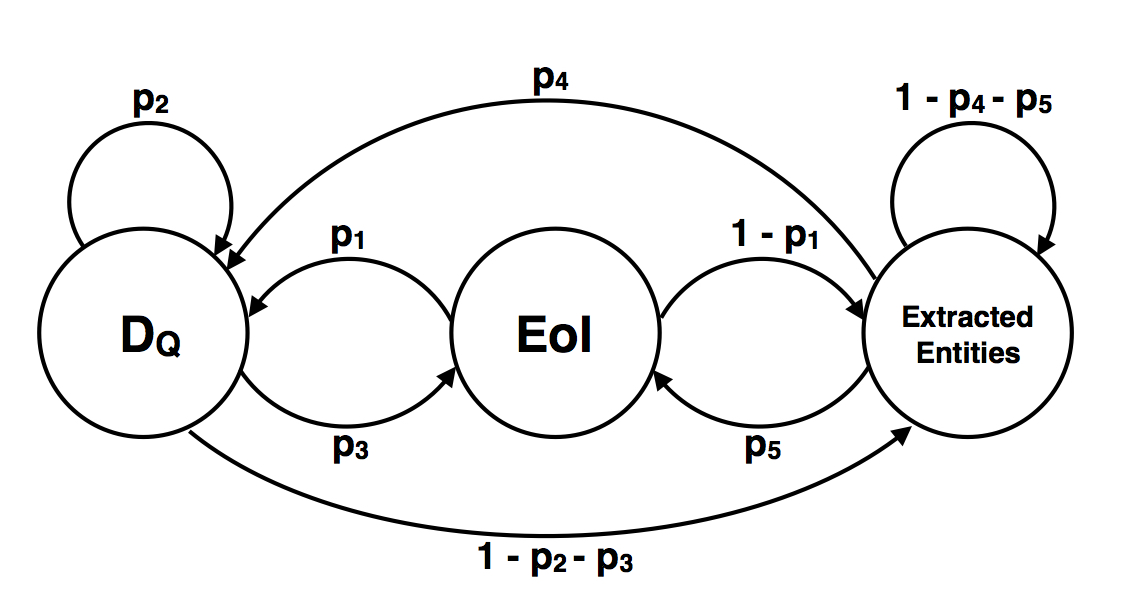
\includegraphics[width=0.95\textwidth]{markov_chain}
\end{mdframed}
	\caption{The Markov chain of the process.}
	\label{fig:markov_chain}
\end{figure}


\subsection{Creating the Graph of States and Transitions}
First, we provide a definition of a semantic graph of documents and entities, 
and then we describe in detail the construction of the graph of states and 
transitions corresponding to the modelling.

\vspace{2mm}\noindent 
{\bf The semantic graph of documents and entities}. Both the documents and 
entities are considered as vertices in $\rchi$, 
and for drawing edges we take into account documents in which an entity
has been detected. Specifically, an edge is drawn starting from an entity $e$ 
and ending at a document $d$, if $e \in ents(d)$ (i.e., e was extracted from d). 
By exploiting a Semantic Knowledge Base (in our case {\em DBpedia}), interesting 
related entities linked as triples with the entity can be fetched 
(performed during {\em entity enrichment} step. In the RDF Graph $G_i$, let $T(u_e) \subseteq G_i$ be triples that describe information about $u_e$. 
Now, for two entities $e_1, e_2 \in E$, if $(u_{e_1}, p, u_{e_2}) \in T(u_e1)$, 
then we draw an edge starting from the entity $e_1$ and ending at the entity $e_2$
and we denote this edge by $edge(e_1, e_2)$.

\begin{figure}[ht]
\begin{mdframed}
	\centering
	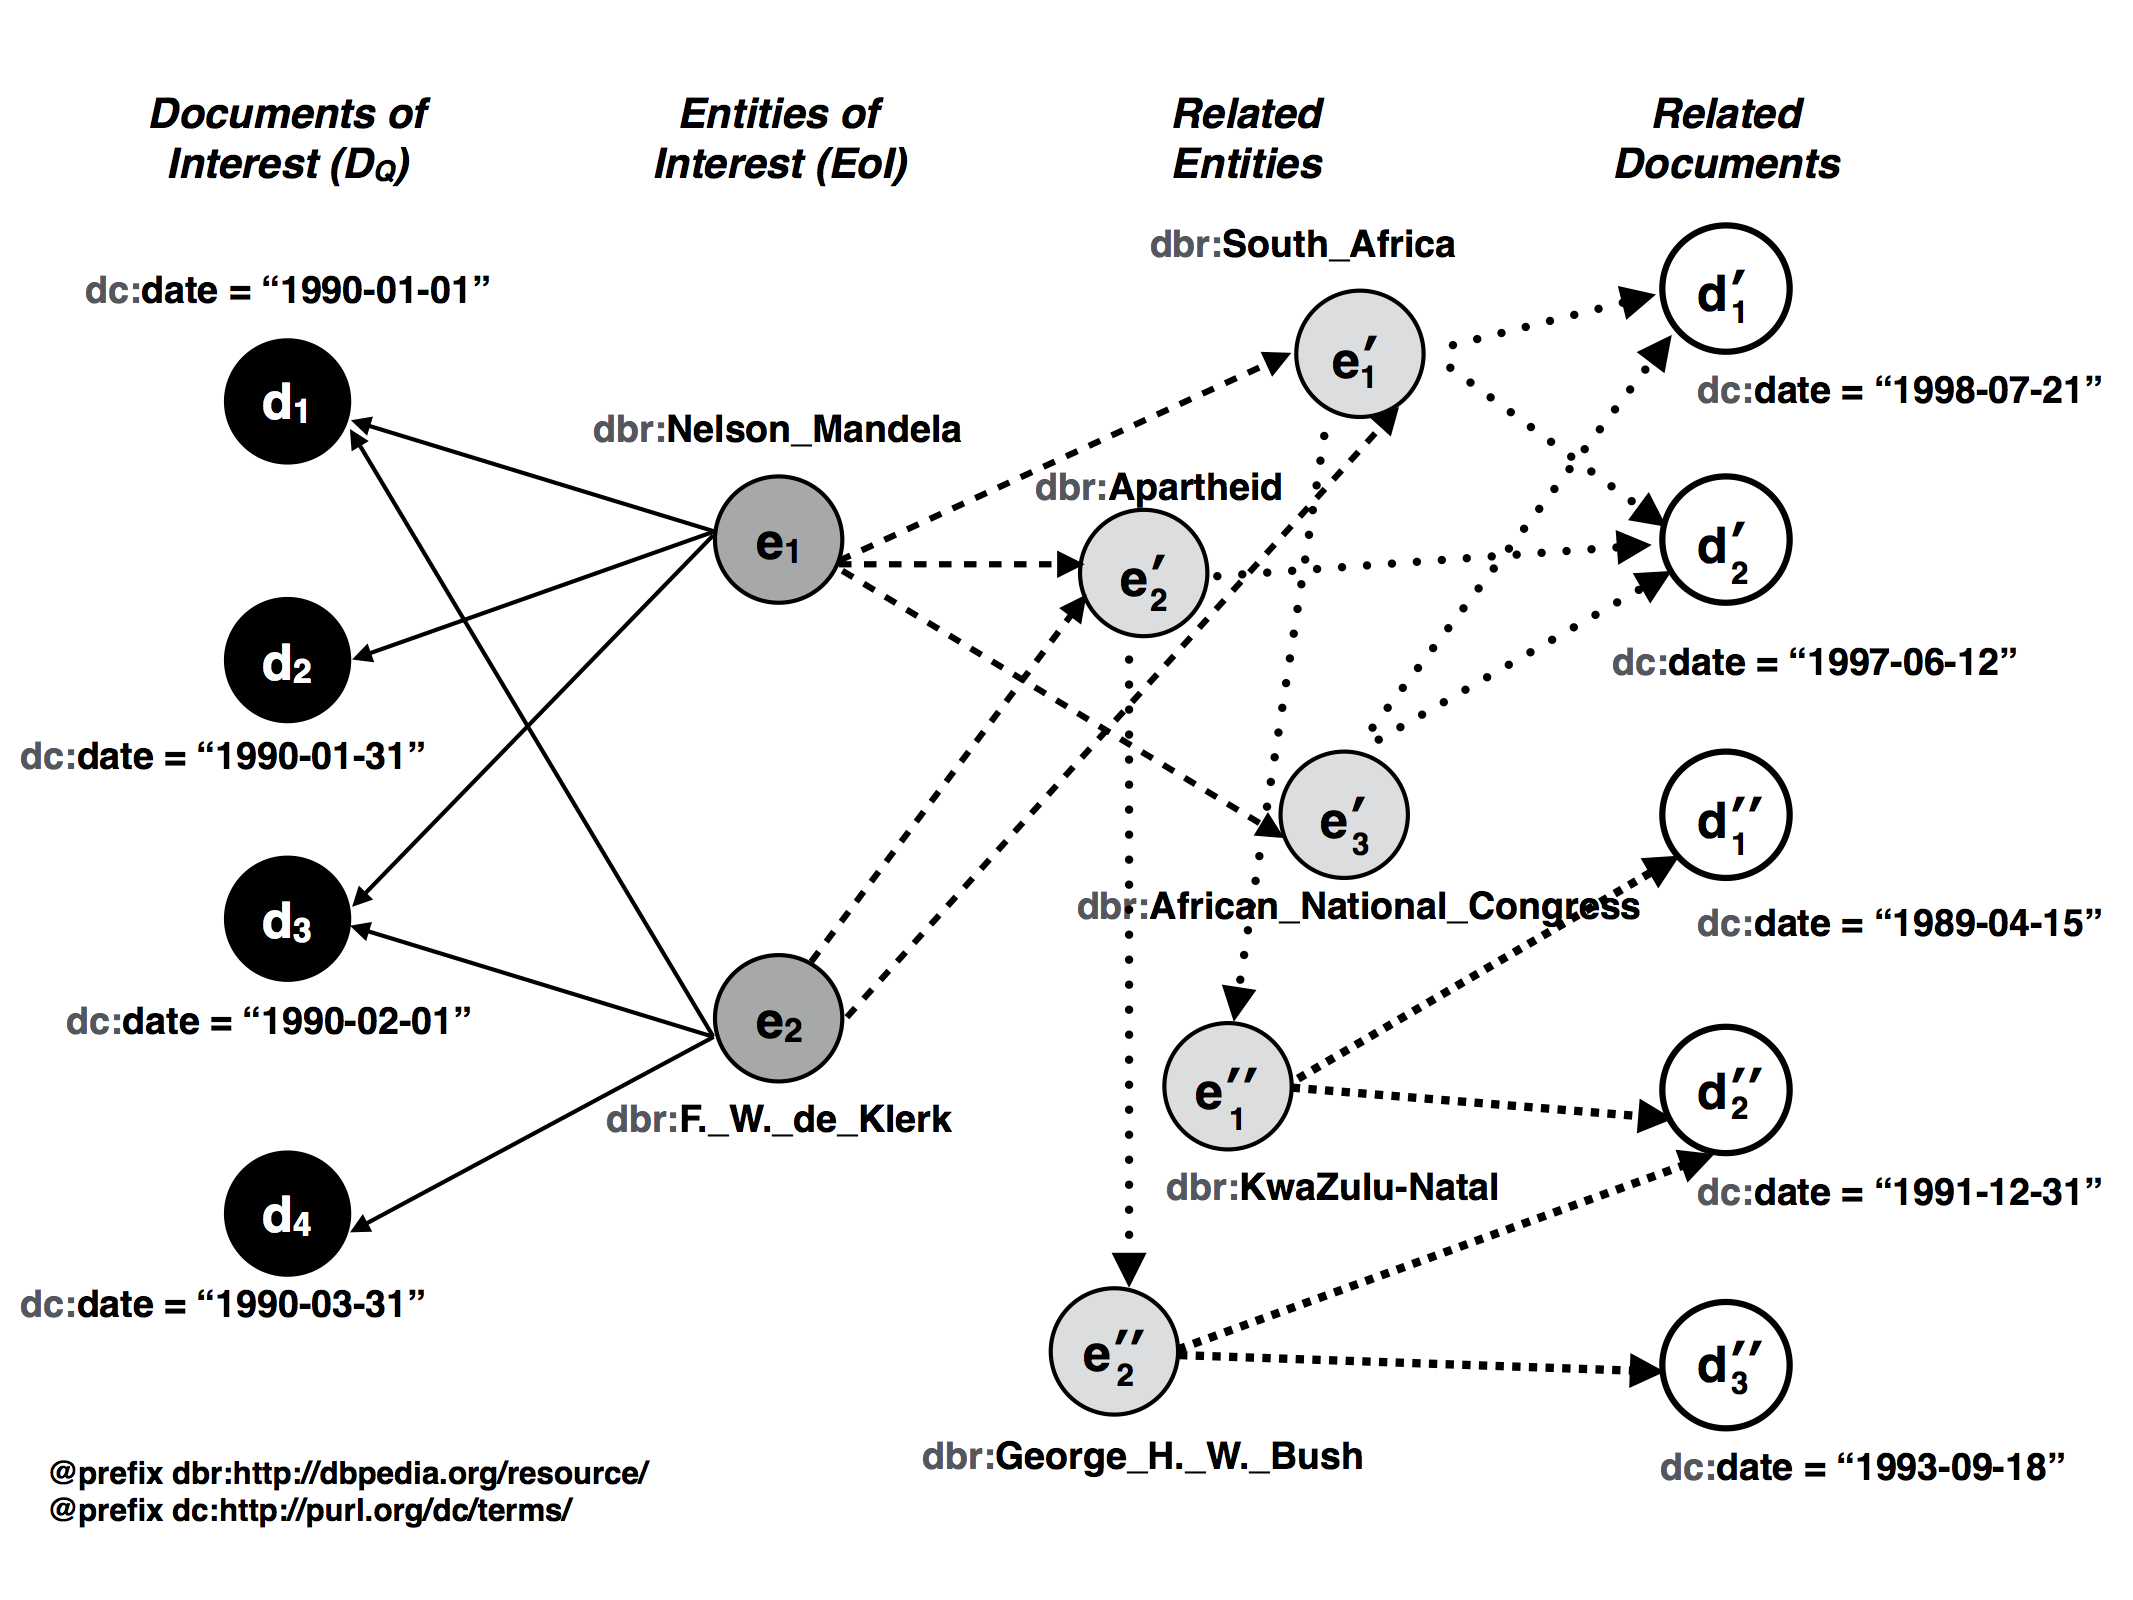
\includegraphics[width=0.95\textwidth]{example_graph}
\end{mdframed}
	\caption{An example of a semantic graph of documents and entities.}
	\label{fig:example_graph}
\end{figure}

\vspace{2mm}\noindent
{\bf The State Transition Graph (STG)}. From $\rchi$ we now define a STG $\mathcal{G} = (\mathcal{E}, \mathcal{P})$. For each node $n$ in $\rchi$, 
we create a node in $\mathcal{G}$. 
For each directed edge $(n \rightarrow n')$ in $\rchi$ 
we create two directed edges in $\mathcal{G}$; 
one of the same direction $(n \rightarrow n')$ and one of the 
opposite direction $(n' \rightarrow n)$. This is done because in our context, 
if a property connects two nodes in $\rchi$, 
then these nodes are {\em semantically biconnected}.   
For example, in case of two entities $e_1$ = \texttt{Sebastian\_Vettel}  
and $e_2$ = \texttt{Scuderia\_Ferrari}, we can either say that $(e_1, "team", e_2)$ 
or that $( e_2, "driver", e_1)$, the difference only being in how we name the property. 

\vspace{2mm}\noindent
{\bf Weighting the edges}. We consider the different scenarios where the walker 
can lie and move to, and specify the weights of the edges. 

\vspace{2mm}\noindent
{\bf Case 1:} The walker lies at an entity of interest $e$ and he moves to 
a document $d \in D_Q$, i.e., the movement is along the edge $n \rightarrow n'$, where
$n=e, e \in E_Q$ and $n'=d, d \in D_Q$. 

Considering relativeness and timeliness, the score of a document $d \in D_Q$ can be defined as: 
\begin{equation}
\begin{split}
\small
ScoreD^{f,t}(d) = Score^{f}(d) \cdot Score^{t}(d) 
\end{split}
\end{equation}
The weight of the edge ($n \rightarrow n'$) in this case ($n=e, n'=d$) for 
both {\tt AND} and {\tt OR} semantics can be defined as:
\begin{equation}
\begin{split}
\small
weight(e \rightarrow d) = \frac{ScoreD^{f,t}(d)}{\sum_{d' \in D_Q}(ScoreD^{f,t}(d'))}  
\end{split}
\end{equation}

\vspace{2mm}\noindent
{\bf Case 2:} The walker lies at an entity of interest $e$ and moves to 
a related entity $e'$. Movement is along the edge ($n \rightarrow n'$) where 
($n=e, n'=e'$). Considering relatedness, for both {\tt AND} and {\tt OR} Semantics
we use the following criteria for assigning weights to the edges: 
\begin{equation}
\begin{split}
\small
weight(e \rightarrow e') = \frac{ScoreE(e')}{\sum_{e' \in E_D \setminus E_Q}(ScoreE(e''))}  
\end{split}
\end{equation}

We also have to take into consideration that the weight of the outgoing edges 
must represent transition probabilities, i.e., they must sum to 1. 
Thus, the weight from an entity-node e to a connected node $n$ can be 
generally defined as:
\begin{gather}
\small
weight(e \rightarrow n) = \begin{cases}
    p_1 \cdot \frac{ScoreD^{f,t}(d)}{\sum_{d' \in D_Q}(ScoreD^{f,t}(d'))} \qquad 
    n = d\\
    (1-p_1) \cdot \frac{ScoreE(e')}{\sum_{e' \in E_D \setminus E_Q}(ScoreE(e''))} 
    \qquad n = e'
\end{cases}
\end{gather}
 

\vspace{2mm}\noindent
Figure \ref{fig:eoi_weighting} shows an example of an STG of documents of interest, 
entities of interest and related entities along with the edges and some of the edge 
weights for the entities of interest. 
The criteria for assigning weight in the first and second case is based upon the 
notion that from an entity of interest a surfer is more likely to move to a document
that mentions the entity of interest many times and is published in important 
time periods (for EoI). It is also likely to move to a related entity that is important
to the EoI.

\begin{figure}[ht]
\begin{mdframed}
	\centering
	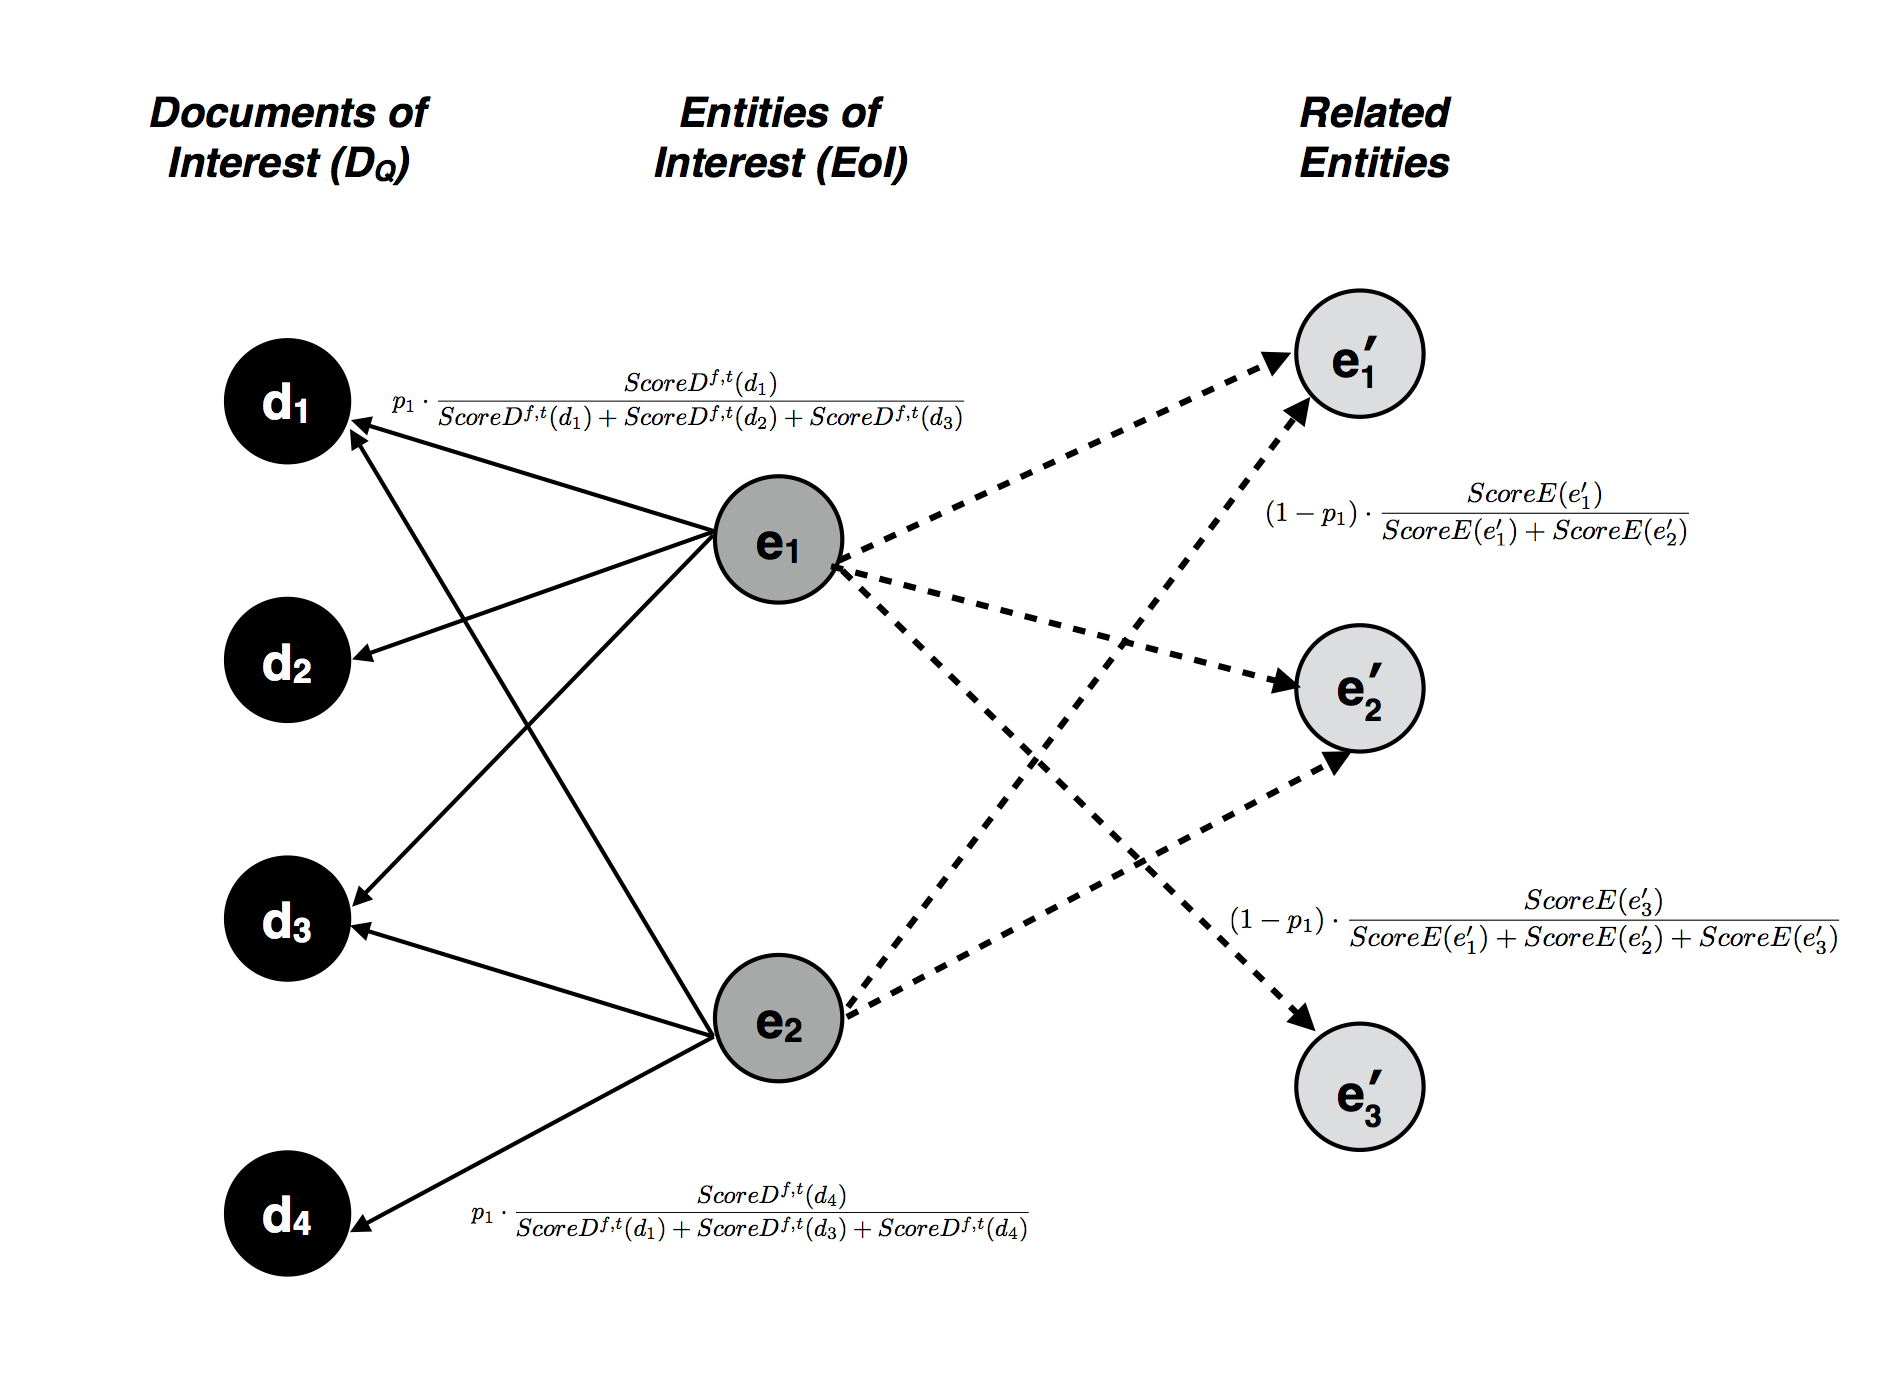
\includegraphics[width=0.95\textwidth]{eoi_weighting}
\end{mdframed}
	\caption{Biasing the link selection from an EoI-node.}
	\label{fig:eoi_weighting}
\end{figure}


\vspace{2mm}\noindent
{\bf Case 3:} The walker is at a document $d$ and moves to another document $d' \in D_Q$, i.e., the walker moves along the edge $n \rightarrow n'$ where $n=d$ and $n'=d'$. 
In this case, we use the following criterion for assigning weight to the edge:
\begin{equation}
\begin{split}
\small
weight(d \rightarrow d') = \frac{ScoreD^{m}(d')}{\sum_{d'' \in D_Q , d'' \neq d}(ScoreD^{m}(d''))}
\end{split}
\end{equation}

\vspace{2mm}\noindent
{\bf Case 4:} The walker is at a document d and moves to an entity of interest e, i.e., 
the movement is along the edge ($n \rightarrow n'$) where $n=d$ and $n'=e$. We do the 
weight assignment in this case as follows:
\begin{equation}
\begin{split}
\small
weight(d \rightarrow e) = \frac{1}{|ents(d) \cap E_Q|}
\end{split}
\end{equation}
This means that we define that it is equiprobable for a walker to move to any of the entities of interest from a document containing the EoI. In case the document mentions 
only one EoI, then weight becomes equal to 1.

\vspace{2mm}\noindent
Like in the first and second case, in these cases as well, the weight of the 
outgoing edges must represent transition probabilities and sum to 1. Hence, we 
define the weight from an entity-node d to a connected node n as:
\begin{gather}
\small
weight(d \rightarrow n) = \begin{cases}
    p_2 \cdot \frac{ScoreD^{m}(d')}{\sum_{d'' \in D_Q , d'' \neq d}(ScoreD^{m}(d''))}
    \qquad n = d'\\
    (1-p_2) \cdot \frac{1}{|ents(d) \cap E_Q|} 
    \qquad n = e
\end{cases}
\end{gather}

\vspace{2mm}\noindent
Figure \ref{fig:doi_weighting} shows an example of an STG graph of documents of interest and entities
of interest along with the edges and 
some of the edge weights for a document of interest.
In the third and fourth case, the criteria for assigning weight is based upon the 
notion that if the surfer is at a document he finds interesting, he would more likely
move to another document closely published (before or after) to it to find out 
more about the event that occurred at the time period. 
For example, a historian stumbling upon an article mentioning about 
Nelson Mandela's release from Victor Vester prison might want to know
more about the details of his release or the events that occurred shortly
before or after his release. 
And if the document is not interesting enough or does not need to be 
explored further, the surfer moves back to one of the entities of interest.    

\begin{figure}[ht]
\begin{mdframed}
	\centering
	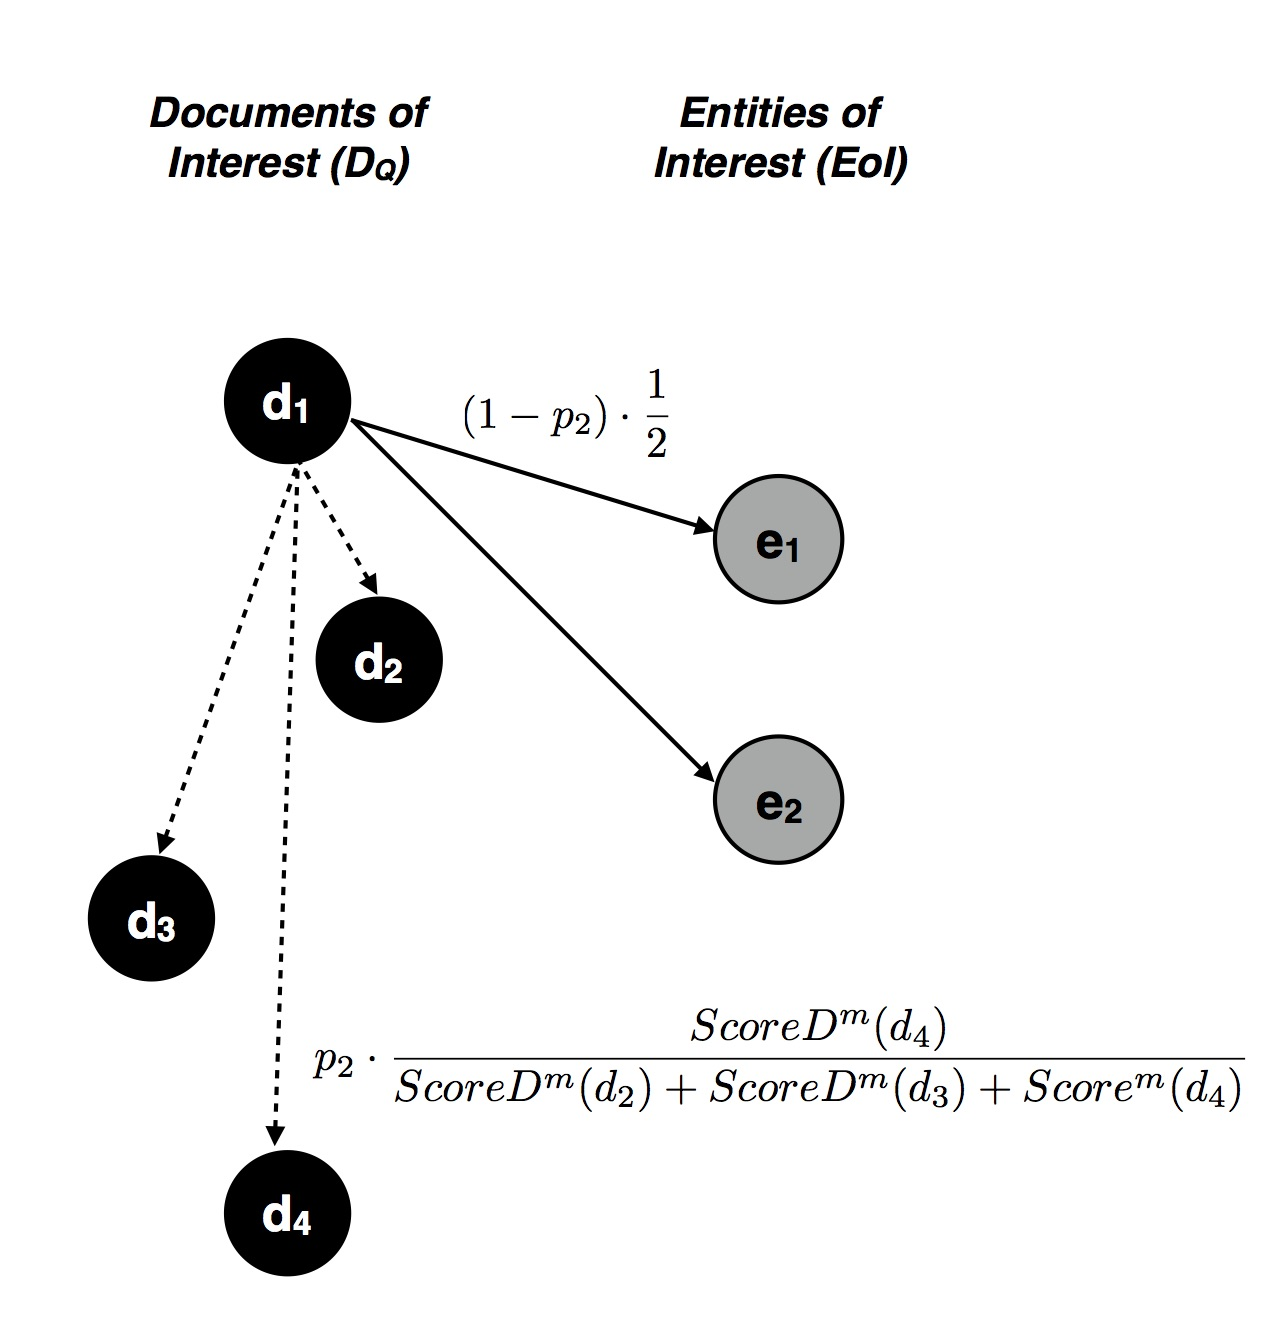
\includegraphics[width=0.5\textwidth]{doi_weighting}
\end{mdframed}
	\caption{Biasing the link selection from a document of interest-node.}
	\label{fig:doi_weighting}
\end{figure}


\vspace{2mm}\noindent
{\bf Case 5:} The walker is at a related entity $e'$ to the EoI and he 
moves to an entity of interest $e$, that is, it travels along the edge 
($n \rightarrow n'$) where $n=e'$ and $n'=e$. 
We define the weight assignment as:         
\begin{equation}
\begin{split}
\small
weight(e' \rightarrow e) = \frac{1}{|edge(e', e'')|} \qquad e'' \in E_Q
\end{split}
\end{equation}
This equation also translates as that there is equal probability for a
walker to move from a related entity $e'$ to any of the entities of interest
connected to it by an edge. In case the related entity is connected to only one 
entity of interest, the weight of the edge becomes 1.

\vspace{2mm}\noindent
{\bf Case 6:} The walker is at a related entity $e'$ and  
moves to a document $d' \in docs(e')$, that is, movement is along the edge 
($n \rightarrow n'$) where $n=e'$ and $n'=d'$. 
We take into consideration relativeness and define the weight assignment as:         
\begin{equation}
\begin{split}
\small
weight(e' \rightarrow d') = \frac{ScoreD^{f}(d')}{\sum_{d'' \in docs(e')}(ScoreD^{f}(d''))} \qquad d' \in docs(e')
\end{split}
\end{equation}
This equation also translates as that there is equal probability for a
walker to move from a related entity $e'$ to any of the entities of interest
connected to it by an edge. In case the related entity is connected to only one 
entity of interest, the weight of the edge becomes 1.

\vspace{2mm}\noindent
{\bf Case 7:} The walker is at a related entity $e'$ and  
moves to another entity $e''$, that is, movement is along the edge 
($n \rightarrow n'$) where $n=e'$ and $n'=e''$. 
Using relatedness we define the weight assignment as:         
\begin{equation}
\begin{split}
\small
weight(e' \rightarrow e'') = \frac{ScoreE(e'')}{\sum_{e''' \in E_D \setminus E_Q}(ScoreE(e'''))} 
\end{split}
\end{equation}
Here we use the same way to assign weight as we did in the second case where
the movement was from an EoI $e$ to a related entity $e'$.

Because the weight of the outgoing edges must sum to 1 as they represent transition
probabilities, we define the weight from a related entity-node e' to a connected 
node n as:
\begin{gather}
\small
weight(e' \rightarrow n) = \begin{cases}
    p_3 \cdot \frac{1}{|edge(e', e'')|} \qquad e'' \in E_Q, n = e\\
    p_4 \cdot \frac{ScoreD^{f}(d')}{\sum_{d'' \in docs(e')}(ScoreD^{f}(d''))} \qquad n= d', d' \in docs(e') \\
    (1-p_3-p_4) \cdot {\frac{ScoreE(e'')}{\sum_{e''' \in E_D \setminus E_Q}(ScoreE(e'''))}} \qquad n = e'',p_3 + p_4 \leq 1
\end{cases}
\end{gather}
Figure \ref{fig:entity_weighting} shows an example of an STG of entities of interest, related entities and 
related documents along with the edges and edge weights for a related entity.
Also, in the case where the walker is at further related entity $e''$ and wants to 
make a transition, the same cases 5, 6 and 7 apply.  

\begin{figure}[ht]
\begin{mdframed}
	\centering
	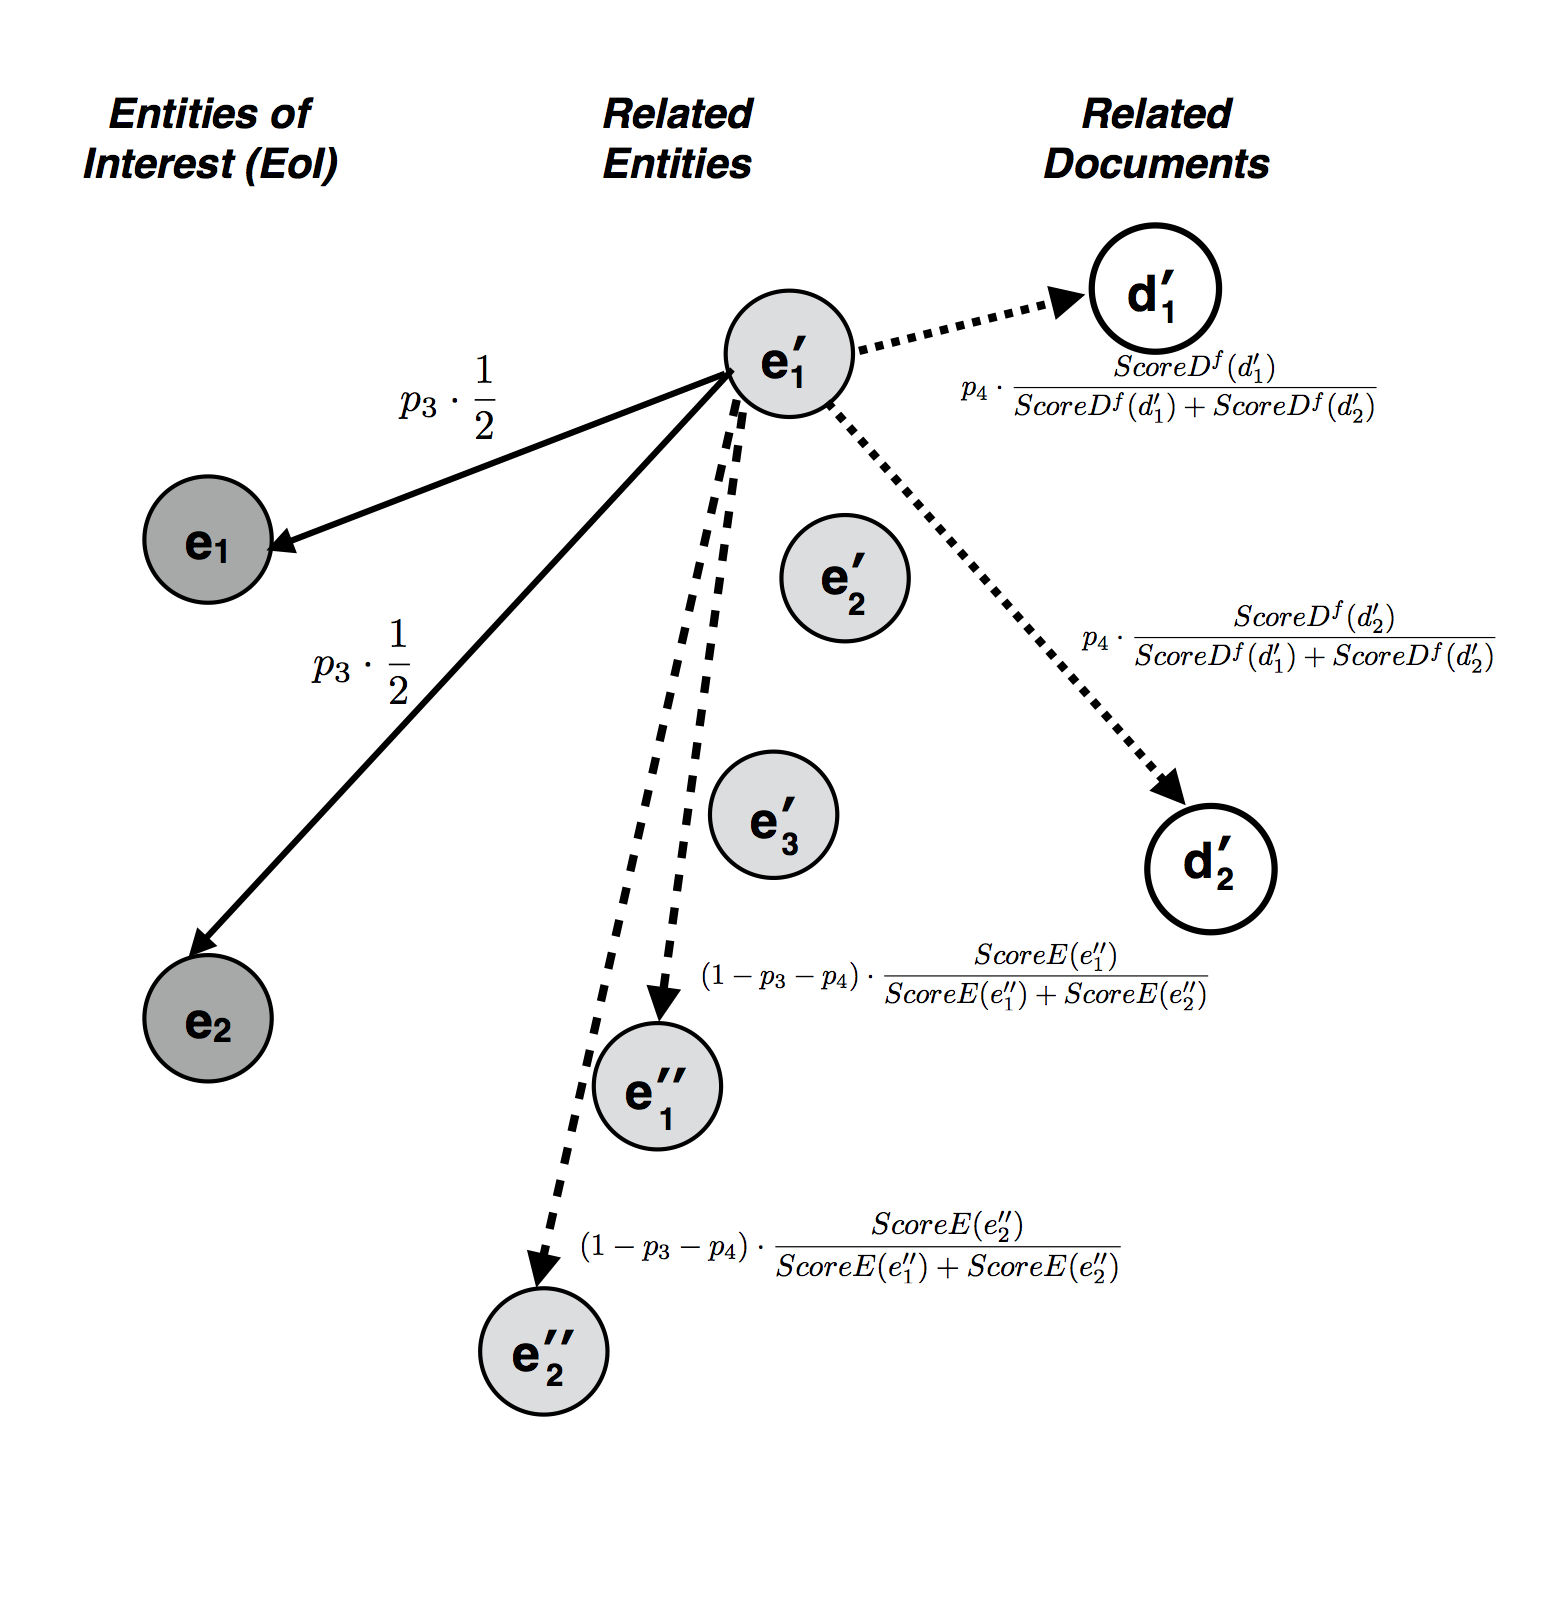
\includegraphics[width=0.75\textwidth]{entities_weighting}
\end{mdframed}
	\caption{Biasing the link selection from a related entity-node.}
	\label{fig:entity_weighting}
\end{figure}

\vspace{2mm}\noindent
{\bf Case 8:} The walker is at a document $d'$ which he has reached from a related
entity $e'$ and now he wants to move back to an entity of interest $e$ and display
the initial results. 

\vspace{2mm}\noindent
This forms a special case because although there may not exist
an edge between the EoI $e$ and the document $d'$ as it may be the case
that $d' \notin docs(e) $. But still we allow this transition as the walker after 
travelling to a document mentioning a related entity he may always choose to reset
and display initial results as his original objective was to find interesting 
documents related to the entities of interest EoI in a specific time period.
In this case, if $\nexists edge(d', e)$ then we create an
$edge (d', e)$ where $e \in E_Q$ 
and the edge direction is from $d'$ to $e$. 
The weight in this case is defined as:
\begin{equation}
\begin{split}
\small
weight(d' \rightarrow e) = \frac{1}{|E_Q|} 
\end{split}
\end{equation}

\vspace{2mm}\noindent
{\bf Case 9:} The walker is at a document $d'$ which he has reached from a related
entity $e'$ and now he moves to an entity $e'$ extracted from it. 
The criterion for assigning weight in this case will be as follows:
\begin{equation}
\begin{split}
\small
weight(d' \rightarrow e') = \frac{1}{|ents(d') \setminus E_Q|} 
\end{split}
\end{equation}
This means that there is an equal probability of the walker to move from 
a document $d'$ to any of the extracted entities except for the entities of 
interest. In case the walker moves from EoI $e$ to a related entity $e'$ and further 
to related entity $e''$ before moving to a document $d''$, the cases 8 and 9 apply.

\vspace{2mm}\noindent
For the transition probabilities in the eighth and ninth case, we need to 
make the sum of all the outgoing edges from $d'$ to be equal to 1. 
Thus, we modify the edge weights from document-node $d'$ to a node $n$ as:
\begin{gather}
\small
weight(d' \rightarrow n) = \begin{cases}
    p_5 \cdot \frac{1}{|E_Q|} \qquad n = e\\
    (1-p_5) \cdot \frac{1}{|ents(d') \setminus E_Q|}\qquad n = e'
\end{cases}
\end{gather}

Figure \ref{fig:document_weighting} shows an example of an STG of
related documents, related entities and entities of interest along with the
edges and their weights for a related document.

\begin{figure}[ht]
\begin{mdframed}
	\centering
	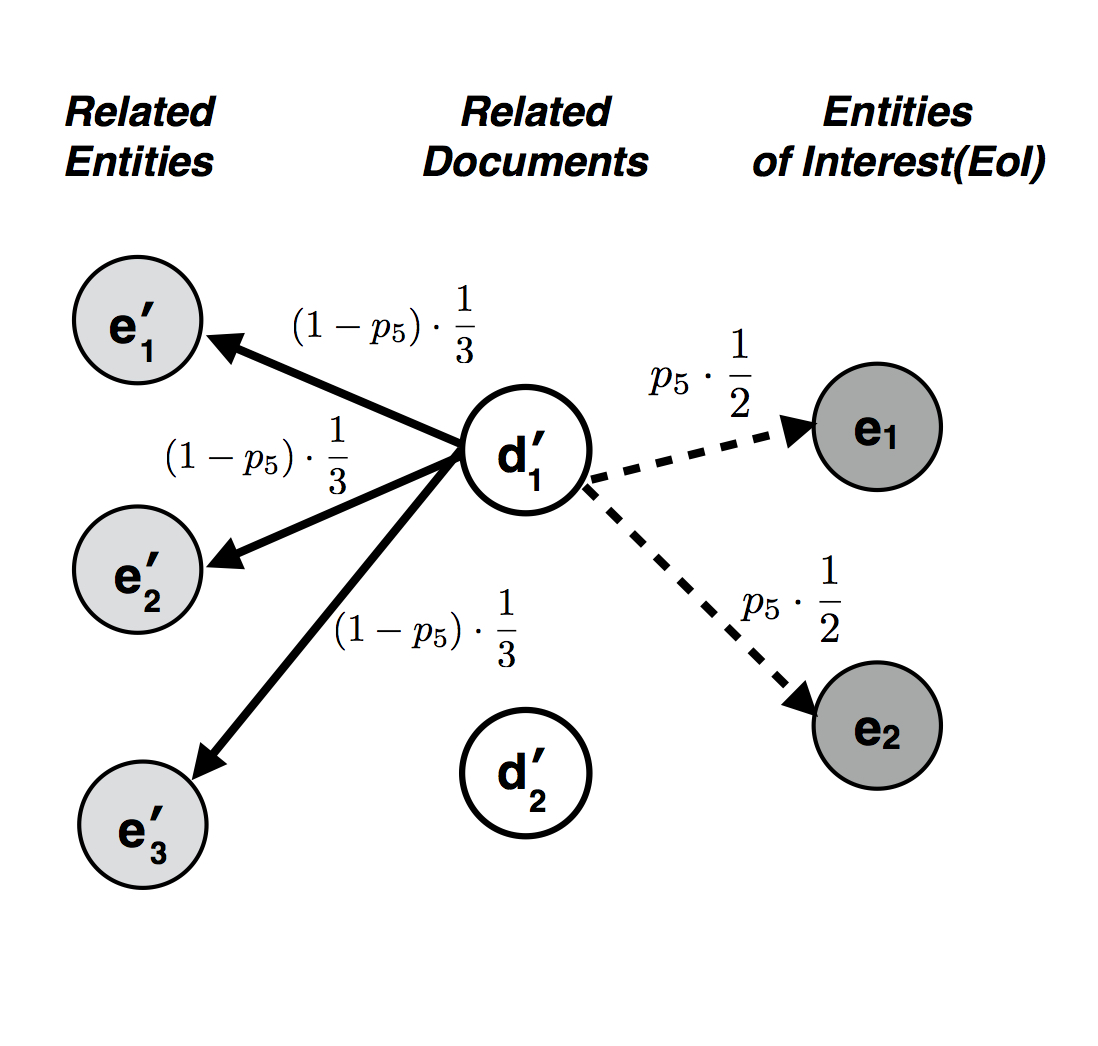
\includegraphics[width=0.5\textwidth]{document_weighting}
\end{mdframed}
	\caption{Biasing the link selection from a related document-node.}
	\label{fig:document_weighting}
\end{figure}


\subsection{Analyzing the STG}
For a node $n$, let $in(n)$ be the set of nodes that point to n. 
The {\em PageRank-like} value $r(n)$ is defined as:
\begin{equation}
\begin{split}
\small
r(n) = d \cdot Jump(n) + (1-d) \cdot \sum_{n' \in in(n)}{(weight(n \rightarrow n') \cdot r(n'))}  
\end{split}
\end{equation}
%continue with describing more about Analyzing the Detail, 
%add pseudo-code for PageRank algorithm if required.
%Describe Random Jumps and tuning the algorithm 

\bibliographystyle{abbrv}
\bibliography{bib/semlayerRanking}

\end{document}